\documentclass[a4paper,11pt,final]{article}
        \usepackage{fancyvrb, color, graphicx, hyperref, amsmath, url, textcomp}
        \usepackage{palatino}
        \usepackage[a4paper,text={16.5cm,25.2cm},centering]{geometry}

        %Set different options for xetex and luatex
        \usepackage{iftex}
        \ifxetex\usepackage{fontspec}\fi

        \ifluatex\usepackage{fontspec}\fi

        \hypersetup
        {   pdfauthor = {Pweave},
            pdftitle={Published from AR_yw.mdw},
            colorlinks=TRUE,
            linkcolor=black,
            citecolor=blue,
            urlcolor=blue
        }
        \setlength{\parindent}{0pt}
        \setlength{\parskip}{1.2ex}
        % fix for pandoc 1.14
        \providecommand{\tightlist}{%
            \setlength{\itemsep}{0pt}\setlength{\parskip}{0pt}}
        
\makeatletter
\def\PY@reset{\let\PY@it=\relax \let\PY@bf=\relax%
    \let\PY@ul=\relax \let\PY@tc=\relax%
    \let\PY@bc=\relax \let\PY@ff=\relax}
\def\PY@tok#1{\csname PY@tok@#1\endcsname}
\def\PY@toks#1+{\ifx\relax#1\empty\else%
    \PY@tok{#1}\expandafter\PY@toks\fi}
\def\PY@do#1{\PY@bc{\PY@tc{\PY@ul{%
    \PY@it{\PY@bf{\PY@ff{#1}}}}}}}
\def\PY#1#2{\PY@reset\PY@toks#1+\relax+\PY@do{#2}}

\expandafter\def\csname PY@tok@gd\endcsname{\def\PY@tc##1{\textcolor[rgb]{0.63,0.00,0.00}{##1}}}
\expandafter\def\csname PY@tok@gu\endcsname{\let\PY@bf=\textbf\def\PY@tc##1{\textcolor[rgb]{0.50,0.00,0.50}{##1}}}
\expandafter\def\csname PY@tok@gt\endcsname{\def\PY@tc##1{\textcolor[rgb]{0.00,0.27,0.87}{##1}}}
\expandafter\def\csname PY@tok@gs\endcsname{\let\PY@bf=\textbf}
\expandafter\def\csname PY@tok@gr\endcsname{\def\PY@tc##1{\textcolor[rgb]{1.00,0.00,0.00}{##1}}}
\expandafter\def\csname PY@tok@cm\endcsname{\let\PY@it=\textit\def\PY@tc##1{\textcolor[rgb]{0.25,0.50,0.50}{##1}}}
\expandafter\def\csname PY@tok@vg\endcsname{\def\PY@tc##1{\textcolor[rgb]{0.10,0.09,0.49}{##1}}}
\expandafter\def\csname PY@tok@m\endcsname{\def\PY@tc##1{\textcolor[rgb]{0.40,0.40,0.40}{##1}}}
\expandafter\def\csname PY@tok@mh\endcsname{\def\PY@tc##1{\textcolor[rgb]{0.40,0.40,0.40}{##1}}}
\expandafter\def\csname PY@tok@go\endcsname{\def\PY@tc##1{\textcolor[rgb]{0.53,0.53,0.53}{##1}}}
\expandafter\def\csname PY@tok@ge\endcsname{\let\PY@it=\textit}
\expandafter\def\csname PY@tok@vc\endcsname{\def\PY@tc##1{\textcolor[rgb]{0.10,0.09,0.49}{##1}}}
\expandafter\def\csname PY@tok@il\endcsname{\def\PY@tc##1{\textcolor[rgb]{0.40,0.40,0.40}{##1}}}
\expandafter\def\csname PY@tok@cs\endcsname{\let\PY@it=\textit\def\PY@tc##1{\textcolor[rgb]{0.25,0.50,0.50}{##1}}}
\expandafter\def\csname PY@tok@cp\endcsname{\def\PY@tc##1{\textcolor[rgb]{0.74,0.48,0.00}{##1}}}
\expandafter\def\csname PY@tok@gi\endcsname{\def\PY@tc##1{\textcolor[rgb]{0.00,0.63,0.00}{##1}}}
\expandafter\def\csname PY@tok@gh\endcsname{\let\PY@bf=\textbf\def\PY@tc##1{\textcolor[rgb]{0.00,0.00,0.50}{##1}}}
\expandafter\def\csname PY@tok@ni\endcsname{\let\PY@bf=\textbf\def\PY@tc##1{\textcolor[rgb]{0.60,0.60,0.60}{##1}}}
\expandafter\def\csname PY@tok@nl\endcsname{\def\PY@tc##1{\textcolor[rgb]{0.63,0.63,0.00}{##1}}}
\expandafter\def\csname PY@tok@nn\endcsname{\let\PY@bf=\textbf\def\PY@tc##1{\textcolor[rgb]{0.00,0.00,1.00}{##1}}}
\expandafter\def\csname PY@tok@no\endcsname{\def\PY@tc##1{\textcolor[rgb]{0.53,0.00,0.00}{##1}}}
\expandafter\def\csname PY@tok@na\endcsname{\def\PY@tc##1{\textcolor[rgb]{0.49,0.56,0.16}{##1}}}
\expandafter\def\csname PY@tok@nb\endcsname{\def\PY@tc##1{\textcolor[rgb]{0.00,0.50,0.00}{##1}}}
\expandafter\def\csname PY@tok@nc\endcsname{\let\PY@bf=\textbf\def\PY@tc##1{\textcolor[rgb]{0.00,0.00,1.00}{##1}}}
\expandafter\def\csname PY@tok@nd\endcsname{\def\PY@tc##1{\textcolor[rgb]{0.67,0.13,1.00}{##1}}}
\expandafter\def\csname PY@tok@ne\endcsname{\let\PY@bf=\textbf\def\PY@tc##1{\textcolor[rgb]{0.82,0.25,0.23}{##1}}}
\expandafter\def\csname PY@tok@nf\endcsname{\def\PY@tc##1{\textcolor[rgb]{0.00,0.00,1.00}{##1}}}
\expandafter\def\csname PY@tok@si\endcsname{\let\PY@bf=\textbf\def\PY@tc##1{\textcolor[rgb]{0.73,0.40,0.53}{##1}}}
\expandafter\def\csname PY@tok@s2\endcsname{\def\PY@tc##1{\textcolor[rgb]{0.73,0.13,0.13}{##1}}}
\expandafter\def\csname PY@tok@vi\endcsname{\def\PY@tc##1{\textcolor[rgb]{0.10,0.09,0.49}{##1}}}
\expandafter\def\csname PY@tok@nt\endcsname{\let\PY@bf=\textbf\def\PY@tc##1{\textcolor[rgb]{0.00,0.50,0.00}{##1}}}
\expandafter\def\csname PY@tok@nv\endcsname{\def\PY@tc##1{\textcolor[rgb]{0.10,0.09,0.49}{##1}}}
\expandafter\def\csname PY@tok@s1\endcsname{\def\PY@tc##1{\textcolor[rgb]{0.73,0.13,0.13}{##1}}}
\expandafter\def\csname PY@tok@kd\endcsname{\let\PY@bf=\textbf\def\PY@tc##1{\textcolor[rgb]{0.00,0.50,0.00}{##1}}}
\expandafter\def\csname PY@tok@sh\endcsname{\def\PY@tc##1{\textcolor[rgb]{0.73,0.13,0.13}{##1}}}
\expandafter\def\csname PY@tok@sc\endcsname{\def\PY@tc##1{\textcolor[rgb]{0.73,0.13,0.13}{##1}}}
\expandafter\def\csname PY@tok@sx\endcsname{\def\PY@tc##1{\textcolor[rgb]{0.00,0.50,0.00}{##1}}}
\expandafter\def\csname PY@tok@bp\endcsname{\def\PY@tc##1{\textcolor[rgb]{0.00,0.50,0.00}{##1}}}
\expandafter\def\csname PY@tok@c1\endcsname{\let\PY@it=\textit\def\PY@tc##1{\textcolor[rgb]{0.25,0.50,0.50}{##1}}}
\expandafter\def\csname PY@tok@kc\endcsname{\let\PY@bf=\textbf\def\PY@tc##1{\textcolor[rgb]{0.00,0.50,0.00}{##1}}}
\expandafter\def\csname PY@tok@c\endcsname{\let\PY@it=\textit\def\PY@tc##1{\textcolor[rgb]{0.25,0.50,0.50}{##1}}}
\expandafter\def\csname PY@tok@mf\endcsname{\def\PY@tc##1{\textcolor[rgb]{0.40,0.40,0.40}{##1}}}
\expandafter\def\csname PY@tok@err\endcsname{\def\PY@bc##1{\setlength{\fboxsep}{0pt}\fcolorbox[rgb]{1.00,0.00,0.00}{1,1,1}{\strut ##1}}}
\expandafter\def\csname PY@tok@mb\endcsname{\def\PY@tc##1{\textcolor[rgb]{0.40,0.40,0.40}{##1}}}
\expandafter\def\csname PY@tok@ss\endcsname{\def\PY@tc##1{\textcolor[rgb]{0.10,0.09,0.49}{##1}}}
\expandafter\def\csname PY@tok@sr\endcsname{\def\PY@tc##1{\textcolor[rgb]{0.73,0.40,0.53}{##1}}}
\expandafter\def\csname PY@tok@mo\endcsname{\def\PY@tc##1{\textcolor[rgb]{0.40,0.40,0.40}{##1}}}
\expandafter\def\csname PY@tok@kn\endcsname{\let\PY@bf=\textbf\def\PY@tc##1{\textcolor[rgb]{0.00,0.50,0.00}{##1}}}
\expandafter\def\csname PY@tok@mi\endcsname{\def\PY@tc##1{\textcolor[rgb]{0.40,0.40,0.40}{##1}}}
\expandafter\def\csname PY@tok@gp\endcsname{\let\PY@bf=\textbf\def\PY@tc##1{\textcolor[rgb]{0.00,0.00,0.50}{##1}}}
\expandafter\def\csname PY@tok@o\endcsname{\def\PY@tc##1{\textcolor[rgb]{0.40,0.40,0.40}{##1}}}
\expandafter\def\csname PY@tok@kr\endcsname{\let\PY@bf=\textbf\def\PY@tc##1{\textcolor[rgb]{0.00,0.50,0.00}{##1}}}
\expandafter\def\csname PY@tok@s\endcsname{\def\PY@tc##1{\textcolor[rgb]{0.73,0.13,0.13}{##1}}}
\expandafter\def\csname PY@tok@kp\endcsname{\def\PY@tc##1{\textcolor[rgb]{0.00,0.50,0.00}{##1}}}
\expandafter\def\csname PY@tok@w\endcsname{\def\PY@tc##1{\textcolor[rgb]{0.73,0.73,0.73}{##1}}}
\expandafter\def\csname PY@tok@kt\endcsname{\def\PY@tc##1{\textcolor[rgb]{0.69,0.00,0.25}{##1}}}
\expandafter\def\csname PY@tok@ow\endcsname{\let\PY@bf=\textbf\def\PY@tc##1{\textcolor[rgb]{0.67,0.13,1.00}{##1}}}
\expandafter\def\csname PY@tok@sb\endcsname{\def\PY@tc##1{\textcolor[rgb]{0.73,0.13,0.13}{##1}}}
\expandafter\def\csname PY@tok@k\endcsname{\let\PY@bf=\textbf\def\PY@tc##1{\textcolor[rgb]{0.00,0.50,0.00}{##1}}}
\expandafter\def\csname PY@tok@se\endcsname{\let\PY@bf=\textbf\def\PY@tc##1{\textcolor[rgb]{0.73,0.40,0.13}{##1}}}
\expandafter\def\csname PY@tok@sd\endcsname{\let\PY@it=\textit\def\PY@tc##1{\textcolor[rgb]{0.73,0.13,0.13}{##1}}}

\def\PYZbs{\char`\\}
\def\PYZus{\char`\_}
\def\PYZob{\char`\{}
\def\PYZcb{\char`\}}
\def\PYZca{\char`\^}
\def\PYZam{\char`\&}
\def\PYZlt{\char`\<}
\def\PYZgt{\char`\>}
\def\PYZsh{\char`\#}
\def\PYZpc{\char`\%}
\def\PYZdl{\char`\$}
\def\PYZhy{\char`\-}
\def\PYZsq{\char`\'}
\def\PYZdq{\char`\"}
\def\PYZti{\char`\~}
% for compatibility with earlier versions
\def\PYZat{@}
\def\PYZlb{[}
\def\PYZrb{]}
\makeatother

        
\title{ AR model using Yule-Walker method}
\author{ Matti Pastell}
\date{ 14.5.2013}

\begin{document}
\maketitle


\begin{Verbatim}[commandchars=\\\{\},frame=single,fontsize=\small, xleftmargin=0.5em]
\PY{k+kn}{from} \PY{n+nn}{scipy} \PY{k+kn}{import} \PY{n}{signal}\PY{p}{,} \PY{n}{linalg}
\PY{k+kn}{import} \PY{n+nn}{numpy} \PY{k+kn}{as} \PY{n+nn}{np}
\PY{k+kn}{import} \PY{n+nn}{matplotlib.pyplot} \PY{k+kn}{as} \PY{n+nn}{plt}

\PY{k}{class} \PY{n+nc}{YW}\PY{p}{(}\PY{n+nb}{object}\PY{p}{)}\PY{p}{:}
    \PY{l+s+sd}{\PYZdq{}\PYZdq{}\PYZdq{}A class to fit AR model using Yule\PYZhy{}Walker method\PYZdq{}\PYZdq{}\PYZdq{}}

    \PY{k}{def} \PY{n+nf}{\PYZus{}\PYZus{}init\PYZus{}\PYZus{}}\PY{p}{(}\PY{n+nb+bp}{self}\PY{p}{,} \PY{n}{X}\PY{p}{)}\PY{p}{:}
        \PY{n+nb+bp}{self}\PY{o}{.}\PY{n}{X} \PY{o}{=} \PY{n}{X} \PY{o}{\PYZhy{}} \PY{n}{np}\PY{o}{.}\PY{n}{mean}\PY{p}{(}\PY{n}{X}\PY{p}{)}
\end{Verbatim}

\section{Calculate autocorrelation}\label{calculate-autocorrelation}

YW method requires that we compute the sample autocorrelation function:

\[r_k = \frac{1}{(n-k)\sigma^2}\sum_{t=1}^{n-k}(X_t - \mu)(X_{t+k} - \mu)\]

\begin{Verbatim}[commandchars=\\\{\},frame=single,fontsize=\small, xleftmargin=0.5em]
    \PY{k}{def} \PY{n+nf}{autocorr}\PY{p}{(}\PY{n+nb+bp}{self}\PY{p}{,} \PY{n}{lag}\PY{o}{=}\PY{l+m+mi}{10}\PY{p}{)}\PY{p}{:}
        \PY{n}{c} \PY{o}{=} \PY{n}{np}\PY{o}{.}\PY{n}{correlate}\PY{p}{(}\PY{n+nb+bp}{self}\PY{o}{.}\PY{n}{X}\PY{p}{,} \PY{n+nb+bp}{self}\PY{o}{.}\PY{n}{X}\PY{p}{,} \PY{l+s}{\PYZsq{}}\PY{l+s}{full}\PY{l+s}{\PYZsq{}}\PY{p}{)}
        \PY{n}{mid} \PY{o}{=} \PY{n}{np}\PY{o}{.}\PY{n}{floor}\PY{p}{(}\PY{n+nb}{len}\PY{p}{(}\PY{n}{c}\PY{p}{)}\PY{o}{/}\PY{l+m+mi}{2}\PY{p}{)}
        \PY{n}{acov} \PY{o}{=} \PY{n}{c}\PY{p}{[}\PY{n}{mid}\PY{p}{:}\PY{n}{mid}\PY{o}{+}\PY{n}{lag}\PY{p}{]}
        \PY{n}{acor} \PY{o}{=} \PY{n}{acov}\PY{o}{/}\PY{n}{acov}\PY{p}{[}\PY{l+m+mi}{0}\PY{p}{]}
        \PY{k}{return}\PY{p}{(}\PY{n}{acor}\PY{p}{)}
\end{Verbatim}

\section{Fit}\label{fit}

Form the Yule-Walker equations \(r = R \Phi\) based on sample
autocorrelation \(r_k\). Notice that the matrix R is a Toeplizt matrix
and it is thus easy to form using \texttt{toeplitz} function from
\texttt{scipy.linalg}.

\[\begin{pmatrix}
    r_1\\
    r_2\\
    \vdots\\
    r_p
  \end{pmatrix}
   =
  \begin{pmatrix}
    r_0      & r_1    & \ldots  & r_{p-1} \\
    r_1    & r_0      & \ldots  & r_{p-2} \\
    \vdots & \vdots & \ddots  & \vdots \\ 
    r_{p-1} & r_{p-2} & \ldots  &  r_0
  \end{pmatrix}
    \begin{pmatrix}
      \phi_1\\
      \phi_2\\
      \vdots\\
      \phi_{p}\\
  \end{pmatrix}\]

And solve simply using: \[\Phi = R^{-1}r\]

\begin{Verbatim}[commandchars=\\\{\},frame=single,fontsize=\small, xleftmargin=0.5em]
    \PY{k}{def} \PY{n+nf}{fit}\PY{p}{(}\PY{n+nb+bp}{self}\PY{p}{,} \PY{n}{p}\PY{o}{=}\PY{l+m+mi}{5}\PY{p}{)}\PY{p}{:}
        \PY{n}{ac} \PY{o}{=} \PY{n+nb+bp}{self}\PY{o}{.}\PY{n}{autocorr}\PY{p}{(}\PY{n}{p}\PY{o}{+}\PY{l+m+mi}{1}\PY{p}{)}
        \PY{n}{R} \PY{o}{=} \PY{n}{linalg}\PY{o}{.}\PY{n}{toeplitz}\PY{p}{(}\PY{n}{ac}\PY{p}{[}\PY{p}{:}\PY{n}{p}\PY{p}{]}\PY{p}{)}
        \PY{n}{r} \PY{o}{=} \PY{n}{ac}\PY{p}{[}\PY{l+m+mi}{1}\PY{p}{:}\PY{n}{p}\PY{o}{+}\PY{l+m+mi}{1}\PY{p}{]}
        \PY{n+nb+bp}{self}\PY{o}{.}\PY{n}{phi} \PY{o}{=} \PY{n}{linalg}\PY{o}{.}\PY{n}{inv}\PY{p}{(}\PY{n}{R}\PY{p}{)}\PY{o}{.}\PY{n}{dot}\PY{p}{(}\PY{n}{r}\PY{p}{)}
\end{Verbatim}

\section{Calculate and plot the
spectrum}\label{calculate-and-plot-the-spectrum}

The spectrum of an AR process is given by:

\[S(f) = \frac{\sigma^2}{|1 - \sum_{k=1}^{p} \phi_k e^{-2\pi ikf}|^2} \]

It can be calcuted easily using \texttt{scipy.signal.freqz}.

\begin{Verbatim}[commandchars=\\\{\},frame=single,fontsize=\small, xleftmargin=0.5em]
    \PY{k}{def} \PY{n+nf}{spectrum}\PY{p}{(}\PY{n+nb+bp}{self}\PY{p}{)}\PY{p}{:}
        \PY{n}{a} \PY{o}{=} \PY{n}{np}\PY{o}{.}\PY{n}{concatenate}\PY{p}{(}\PY{p}{[}\PY{n}{np}\PY{o}{.}\PY{n}{ones}\PY{p}{(}\PY{l+m+mi}{1}\PY{p}{)}\PY{p}{,} \PY{o}{\PYZhy{}}\PY{n+nb+bp}{self}\PY{o}{.}\PY{n}{phi}\PY{p}{]}\PY{p}{)}
        \PY{n}{w}\PY{p}{,} \PY{n}{h} \PY{o}{=} \PY{n}{signal}\PY{o}{.}\PY{n}{freqz}\PY{p}{(}\PY{l+m+mi}{1}\PY{p}{,} \PY{n}{a}\PY{p}{)}
        \PY{n}{h\PYZus{}db} \PY{o}{=} \PY{l+m+mi}{10}\PY{o}{*}\PY{n}{np}\PY{o}{.}\PY{n}{log10}\PY{p}{(}\PY{l+m+mi}{2}\PY{o}{*}\PY{p}{(}\PY{n}{np}\PY{o}{.}\PY{n}{abs}\PY{p}{(}\PY{n}{h}\PY{p}{)}\PY{o}{/}\PY{n+nb}{len}\PY{p}{(}\PY{n}{h}\PY{p}{)}\PY{p}{)}\PY{p}{)}
        \PY{n}{plt}\PY{o}{.}\PY{n}{plot}\PY{p}{(}\PY{n}{w}\PY{o}{/}\PY{n}{np}\PY{o}{.}\PY{n}{pi}\PY{p}{,} \PY{n}{h\PYZus{}db}\PY{p}{)}
        \PY{n}{plt}\PY{o}{.}\PY{n}{xlabel}\PY{p}{(}\PY{l+s}{r\PYZsq{}}\PY{l+s}{Normalized Frequency (\PYZdl{}}\PY{l+s}{\PYZbs{}}\PY{l+s}{times }\PY{l+s}{\PYZbs{}}\PY{l+s}{pi\PYZdl{}rad/sample)}\PY{l+s}{\PYZsq{}}\PY{p}{)}
        \PY{n}{plt}\PY{o}{.}\PY{n}{ylabel}\PY{p}{(}\PY{l+s}{r\PYZsq{}}\PY{l+s}{Power/frequency (dB/rad/sample)}\PY{l+s}{\PYZsq{}}\PY{p}{)}
        \PY{n}{plt}\PY{o}{.}\PY{n}{title}\PY{p}{(}\PY{l+s}{r\PYZsq{}}\PY{l+s}{Yule\PYZhy{}Walker Spectral Density Estimate}\PY{l+s}{\PYZsq{}}\PY{p}{)}
\end{Verbatim}

\section{Try it out:}\label{try-it-out}

\begin{Verbatim}[commandchars=\\\{\},frame=single,fontsize=\small, xleftmargin=0.5em]
\PY{o}{\PYZgt{}\PYZgt{}}\PY{o}{\PYZgt{}} \PY{n}{x} \PY{o}{=} \PY{n}{np}\PY{o}{.}\PY{n}{sin}\PY{p}{(}\PY{n}{np}\PY{o}{.}\PY{n}{linspace}\PY{p}{(}\PY{l+m+mi}{0}\PY{p}{,} \PY{l+m+mi}{20}\PY{p}{)}\PY{p}{)}
\PY{o}{\PYZgt{}\PYZgt{}}\PY{o}{\PYZgt{}} \PY{n}{ar1} \PY{o}{=} \PY{n}{YW}\PY{p}{(}\PY{n}{x}\PY{p}{)}
\PY{o}{\PYZgt{}\PYZgt{}}\PY{o}{\PYZgt{}} \PY{n}{ar1}\PY{o}{.}\PY{n}{fit}\PY{p}{(}\PY{p}{)}
\PY{o}{\PYZgt{}\PYZgt{}}\PY{o}{\PYZgt{}} \PY{n}{ar1}\PY{o}{.}\PY{n}{phi}
\PY{n}{array}\PY{p}{(}\PY{p}{[} \PY{l+m+mf}{1.19379795}\PY{p}{,} \PY{o}{\PYZhy{}}\PY{l+m+mf}{0.21810471}\PY{p}{,} \PY{o}{\PYZhy{}}\PY{l+m+mf}{0.12747881}\PY{p}{,} \PY{o}{\PYZhy{}}\PY{l+m+mf}{0.06257484}\PY{p}{,}
\PY{o}{\PYZhy{}}\PY{l+m+mf}{0.12929761}\PY{p}{]}\PY{p}{)}
\PY{o}{\PYZgt{}\PYZgt{}}\PY{o}{\PYZgt{}} \PY{n}{ar1}\PY{o}{.}\PY{n}{spectrum}\PY{p}{(}\PY{p}{)}
\end{Verbatim}
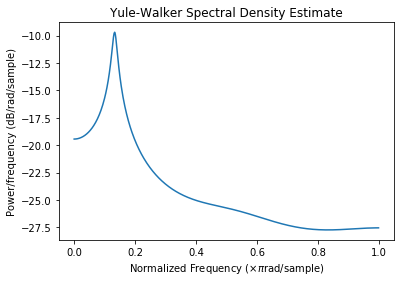
\includegraphics[width= \linewidth]{figures/AR_yw_figure5_1.pdf}


\end{document}